\chapter{Perancangan}
\label{perancangan} 

\section{Struktur Proyek Moodle Mobile}
\label{struktur proyek}

Proyek Moodle Mobile terdiri dari kumpulan file-file dan direktori-direktori utama yang mengandung fungsi dan \textit{source code} untuk aplikasi Moodle Mobile, platform Android dan iOS, alat untuk mebangun perangkat lunak, dan konfigurasi. Struktur dapat dilihat pada Gambar \ref{fig:project-directory}.
\begin{figure} [H]
	\centering  
	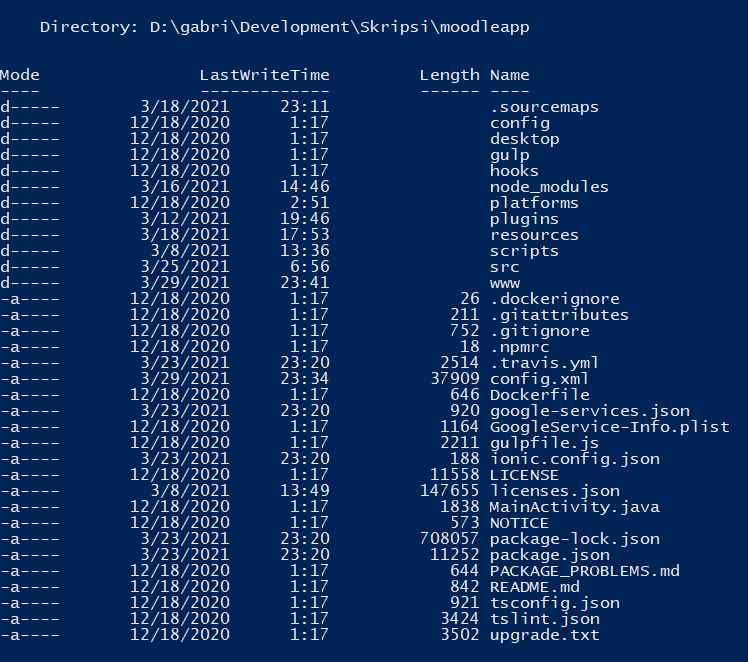
\includegraphics[scale=0.5]{project-directory.PNG}  
	\caption[Struktur direktori proyek Moodle Mobile] {Struktur direktori proyek Moodle Mobile}
	\label{fig:project-directory} 
\end{figure}  

Perubahan pada proyek akan sering dilakukan pada direktori \texttt{src}, dan \texttt{config.xml}. Direktori \texttt{src} berisi kode-kode utama dari aplikasi Moodle mobile dan konfigurasinya. Konfigurasi dari Moodle mobile sendiri diatur oleh file \texttt{config.json} di dalam folder \texttt{src}. File \texttt{Config.xml} berfungsi untuk mengatur konfigurasi dari aplikasi Cordova. Dikarenakan Moodle mobile menggunakan Cordova maka pengaturan saat melakukan \textit{build} untuk perangkat bergerak akan diambil dari file \texttt{Config.xml}. 

Perubahan juga akan terjadi pada direktori \texttt{resources} dan file \texttt{ionic.config.json}. Direktori \texttt{resource} menyimpan sumber untuk ikon dan \textit{splashscreen} yang akan digunakan oleh aplikasi ketika di-\textit{build} untuk platform Android maupun iOS. File \texttt{ionic.config.json} adalah file konfigurasi yang digunakan oleh  Ionic CLI (\textit{Comman Line Interface}), dimana nama aplikasi dan identifikasi aplikasi akan disimpan disana dan dirujuk oleh Ionic CLI ketika digunakan.

Direktori \texttt{node\_modules} juga akan mengalami perubahan namun jarang dilakukan perubahan secara langsung. Dikarenakan direktori tersebut menyimpan \textit{packages} yang dikelola oleh npm. Perubahan yang akan terjadi pada folder \texttt{node\_modules} adalah perubahan seperti yang dibahas di subbab \ref{moodle docs:env}.

\subsection{Perubahan pada \texttt{Config.xml}}
Perubahan pada file \texttt{Config.xml} akan berpengaruh ketika Cordova membangun aplikasi untuk Android dan iOS karena file \texttt{Config.xml} mengatur aturan dan \textit{resource} apa saja yang akan digunakan oleh aplikasi di kedua platform tersebut. 

Perubahan yang dilakukan di dalam file ini adalah sebagai berikut : 

\begin{itemize}
\item Versi aplikasi untuk Android dan iOS akan dimulai dengan versi 1.0.0
\item Nama dari aplikasi adalah \textbf{IDE UNPAR Mobile}
\item Deskripsi aplikasi adalah \textbf{IDE UNPAR app}
\item Penulis aplikasi adalah \textbf{Gabriel Panji Lazuardi} dengan email \textbf{73160068@student.unpar.ac.id}
\item Ikon yang akan digunakan oleh aplikasi dalam platform Android dan iOS.
\item \textit{Splashscreen} yang akan digunakan aplikasi dalam platform Android dan iOS.
\end{itemize}  

\subsection{Perubahahn pada direktori \texttt{src}}

Karena direktori ini mengandung \textit{source code} utama dari aplikasi, seluruh perubahan yang bersifat menambah, mengubah ataupun mengahpus fungsi di dalam aplikasi akan terjadi di dalam direktori \texttt{src}. Seluruh fungsi utama aplikasi terletak pada direktori \texttt{src/core}. Untuk pengaturan tema dari aplikasi terletak pada direktori \texttt{src/theme}. Dan folder \texttt{src/app} mengandung \textit{source code} yang akan dijalankan secara \textit{native} pada platform Android dan iOS seperti mengatur warna dari \textit{status bar}.	

